\documentclass[a4paper]{article}
\usepackage{amsmath}  % Pacote necessário para \dfrac
\usepackage[utf8]{inputenc}
\usepackage[portuguese]{babel}
\usepackage{graphicx}
\usepackage{array}
\usepackage{fancyhdr}
\usepackage{lastpage} % pacote para obter o número total de páginas
\usepackage{geometry} % pacote para ajustar as margens
\usepackage[datesep=/,style=ddmmyyyy]{datetime2} % pacote para formatar a data
\usepackage{setspace} % Inclui o pacote setspace
\usepackage{enumitem}
\usepackage{amssymb} % Para mais símbolos
\usepackage{indentfirst}
\usepackage{hyperref}
\usepackage{array}
\usepackage{booktabs}

\usepackage{titlesec} % Inclui o pacote titlesec
% Redefinindo o formato do título da seção com um tamanho de fonte menor
\titleformat{\section}
{\normalfont\large\bfseries}{\thesection}{1em}{}

% Definindo margens da página e do cabeçalho
\geometry{
	left=20mm,
	right=20mm,
	top=40mm,
	bottom=30mm,
	headsep=20mm
}

\pagestyle{fancy}
\fancyhf{} % limpa o cabeçalho e rodapé padrão
\renewcommand{\headrulewidth}{0pt} % remove a linha do cabeçalho
\renewcommand{\footrulewidth}{0.4pt} % linha acima do rodapé

\fancyhead[C]{ % conteúdo centralizado no cabeçalho
	\begin{tabular}{|m{3.5cm}|m{9.0cm}|m{3.5cm}|}
		\hline
		\begin{minipage}[c][2.0cm][c]{3.5cm}
			\centering
			
\includegraphics[width=2.98cm,height=1.25cm]{logo.png}
		\end{minipage} & 
		\begin{minipage}[c][2.0cm][c]{9cm}
			\centering
			\hyphenpenalty=10000 % Evita hifenização
			\vspace*{\fill} % Espaço vertical flexível antes do texto
			\begin{spacing}{1.5} % Aumenta o espaçamento entre linhas para 1.25
				{\large \textbf{Indutor para Redução de Corrente Transitória \textit{Inrush} em Capacitores}}
			\end{spacing}
			\vspace*{\fill} % Espaço vertical flexível depois do texto
		\end{minipage} & 
		\begin{minipage}[c][2.0cm][c]{3.5cm}
			\raggedleft
			Emissão: \DTMtoday \\
			Folha: \thepage/\pageref{LastPage}
		\end{minipage} \\
		\hline
	\end{tabular}
}


% Conteúdo do rodapé
\fancyfoot[L]{%
	\begin{tabular}[b]{@{}l@{}}
		\href{http://www.dax.energy}{www.dax.energy}
	\end{tabular}
}
\fancyfoot[C]{%
	\begin{tabular}[b]{@{}c@{}}
		\href{mailto:comercial@dax.energy}{comercial@dax.energy}
	\end{tabular}
}
\fancyfoot[R]{%
	\begin{tabular}[b]{@{}r@{}}
		+55 41 99940-3744 \\ 3626-2072
	\end{tabular}
}


\begin{document}
\setstretch{1.25} % Define o espaçamento entre linhas para 1.25

\section{Contexto}
A energização de um banco de capacitores (Figura \ref{fig:picture1}) pelo fechamento de um disjuntor resultará em uma alta corrente de pico transitória (Figura \ref{fig:picture2}), denominada inrush. A magnitude e frequência desta corrente de pico transitória são funções:
\begin{itemize}[label=\textendash]
\item	da tensão aplicada (ponto na onda de tensão no fechamento);
\item	da capacitância equivalente do circuito;
\item	da indutância no circuito (quantidade e localização);
\item	da carga no banco de capacitores no instante de fechamento;
\item	de qualquer amortecimento do circuito devido a resistores de fechamento ou outra resistência no circuito.
\end{itemize}
	
\section{Dados de entrada do banco}
\begin{itemize}[label=\textendash]
	\item	Potencia reativa  = {{potencia_reativa_do_banco}}
	\item	Tensão trifásica  = {{tensao_trifasica}}
	\item	Tensão monofásica  = {{tensao_monofasica}}
	\item	Corrente de curto-circuito  = {{corrente_de_curto}}
\end{itemize}

\begin{center}
	% INSERT_TABLE_HERE
\end{center}



	
	
\section{Considerações Iniciais}

A corrente \textit{inrush} transitória não é um fator limitante em aplicações de bancos de capacitores isolados. Contudo, quando os bancos de capacitores são comutados \textit{back-to-back}, ou seja, quando um banco é acionado enquanto outro banco está conectado ao mesmo barramento, correntes transitórias de altas magnitude e frequência natural irão fluir entre o banco acionado e os que já estavam acionados.

	
\begin{figure}[!hbp]
	\centering
	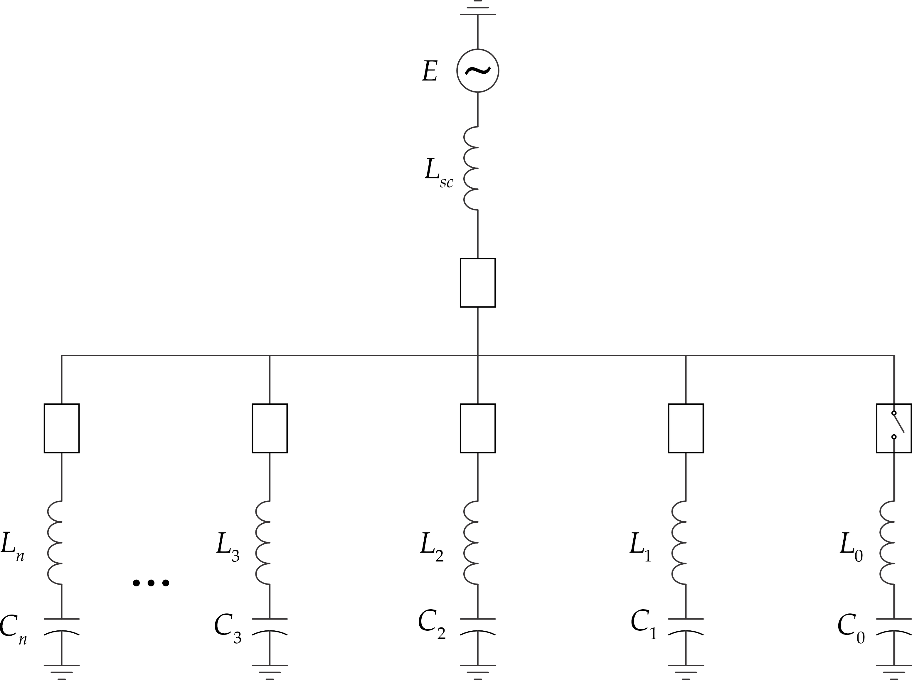
\includegraphics{Picture1.png}
	\caption{Sistema de banco de capacitores.}
	\label{fig:picture1}
\end{figure}


Essa corrente oscilatória é limitada apenas pela impedância do banco de capacitores e pelo circuito entre o banco ou bancos energizados e o banco comutado (Banco \#0), que geralmente decai para zero em uma fração de um ciclo da frequência do sistema. No caso de comutação \textit{back-to-back}, o componente fornecido pela fonte está em uma frequência mais baixa (60 Hz) e tão pequena quando comparada a corrente \textit{inrush}, que pode ser desprezada \href{https://ieeexplore.ieee.org/document/7035261}{[ANSI/IEEE C37.012-1979]}.



\section{Resultados}
\begin{figure}[!hbp]
	\centering
	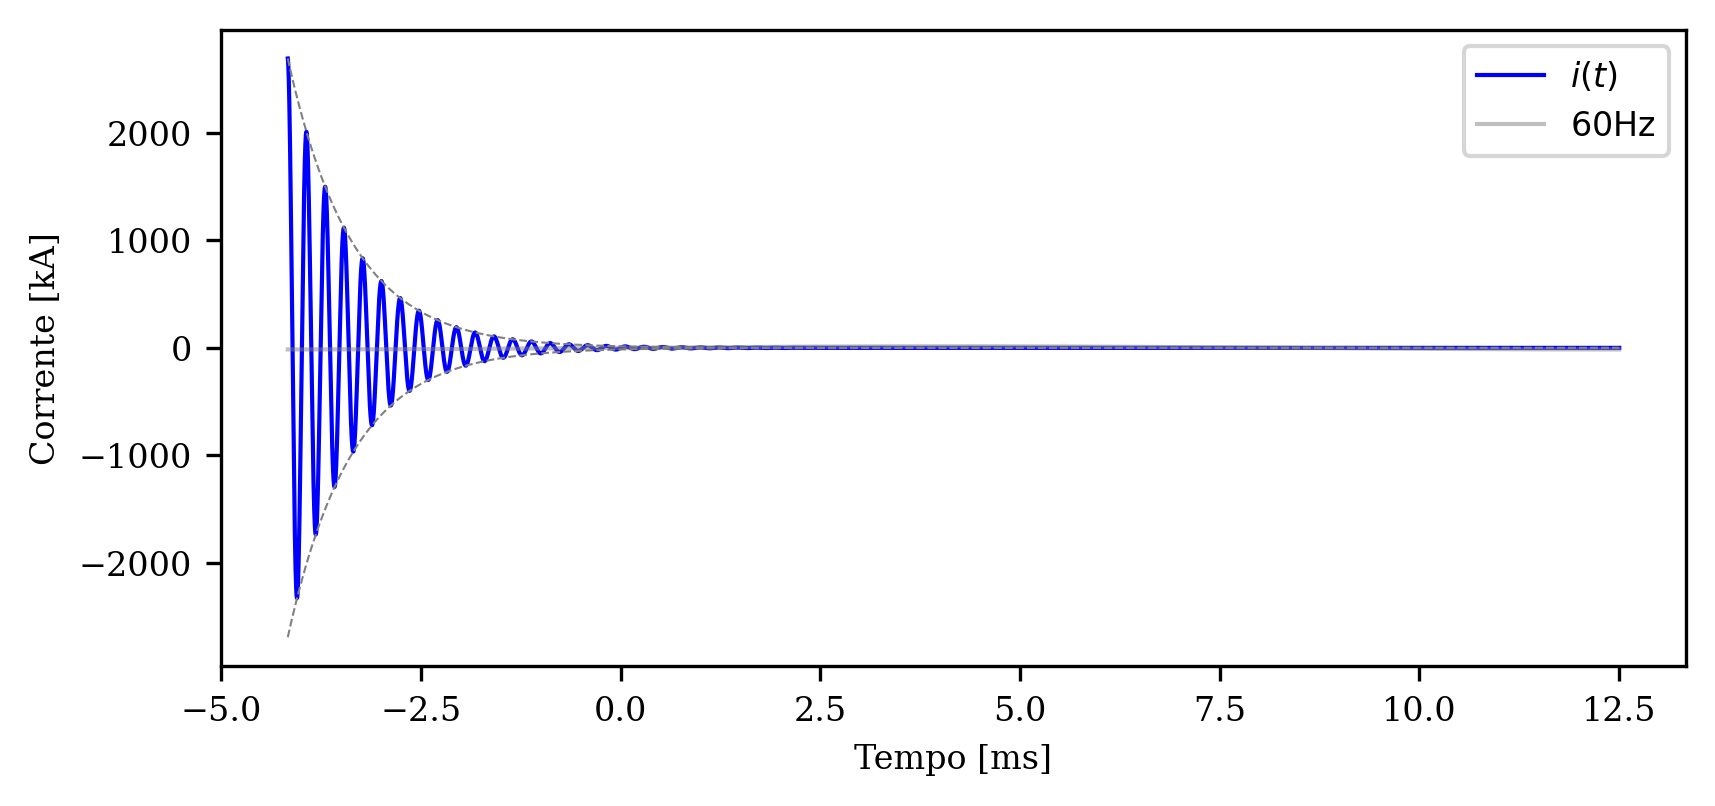
\includegraphics{Correntes.png}
	\caption{Corrente instantânea no banco de capacitores acionado em um ciclo da frequência fundamental.}
	\label{fig:picture2}
\end{figure}

São os valores obtidos com o reator escolhido ($L_{reator} = {{indutancia_escolhida}} \, \mu \rm{H} $):
\begin{itemize}[label=\textendash]
	\item	Corrente de pico: {{corrente_pico}};
	\item	Frequência de Oscilação: {{frequencia_oscilacao}}Hz;
	\item	Corrente inrush / Corrente nominal: {{inrush_inominal}}
\end{itemize}

\section{Conclusão}
{{conclusao1}}

\section{Referências}

\noindent
\begin{tabular}{p{0.2cm} p{15.8cm}}
    \href{https://ieeexplore.ieee.org/document/7035261}{[1]} &
    \begin{minipage}[t]{15.8cm}
        IEEE Application Guide for Capacitance Current Switching for AC High-Voltage Circuit Breakers Rated on a Symmetrical Current Basis, in ANSI/IEEE C37.012-1979, vol., no., pp.1-54, 6 Feb. 1979, doi: 10.1109/IEEESTD.1979.7035261.
    \end{minipage} \\

    \href{https://ieeexplore.ieee.org/document/9574631}{[2]} &
    \begin{minipage}[t]{15.8cm}
        IEEE Approved Draft Standard Requirements for Capacitor Switches for AC Systems (1 kV to 38 kV), in IEEE PC37.66/D10, October 2021, vol., no., pp.1-35, 13 Dec. 2021.
    \end{minipage} \\


    \href{https://webstore.iec.ch/publication/62785}{[3]} &
    \begin{minipage}[t]{15.8cm}
       IEC 62271-100 High-voltage switchgear and controlgear - Part 100: Alternating-current circuit-breakers
    \end{minipage} \\

    \href{https://ieeexplore.ieee.org/document/5318709}{[4]} &
    \begin{minipage}[t]{15.8cm}
        IEEE Standard for AC High-Voltage Circuit Breakers Rated on a Symmetrical Current Basis--Preferred Ratings and Related Required Capabilities for Voltages Above 1000 V, in IEEE Std C37.06-2009, vol., no., pp.1-56, 6 Nov. 2009, doi: 10.1109/IEEESTD.2009.5318709.
    \end{minipage} \\

    \href{https://cdn.standards.iteh.ai/samples/101972/4e7e06bd66d2443da668b8e0c6c60512/IEC-62271-100-2021.pdf}{[5]} &
    \begin{minipage}[t]{15.8cm}
        IEC 62271-100 High-voltage switchgear and controlgear – Part 100: Alternating-current circuit-breakers.
    \end{minipage} \\

    \href{https://www.normas.com.br/autorizar/visualizacao-nbr/313/identificar/visitante}{[6]} &
    \begin{minipage}[t]{15.8cm}
        NBR 5282 Capacitores de potência em derivação para sistema de tensão nominal acima de 1000 V.
    \end{minipage} \\
\end{tabular}



% Espaço para assinaturas
\noindent % Evita a indentação
\begin{minipage}[t]{0.5\textwidth} % Inicia a primeira coluna para assinatura
	\centering % Alinha o texto ao centro
	\vspace{5cm} % Espaço reservado para a assinatura
	\rule{6cm}{0.4pt}\\ % Linha para assinatura
	\textbf{Angelo A. Hafner}\\ % Nome
	Engenheiro Eletricista\\ % Título
	CONFEA: 2.500.821.919\\ % Número do registro
	CREA/SC: 045.776-5\\ % Outro número do registro
	aah@dax.energy % E-mail
\end{minipage}%
\hfill % Espaço entre as colunas
\begin{minipage}[t]{0.5\textwidth} % Inicia a segunda coluna para assinatura
	\centering % Alinha o texto ao centro
	\vspace{5cm} % Espaço reservado para a assinatura
	\rule{6cm}{0.4pt}\\ % Linha para assinatura
	\textbf{Tiago Machado}\\ % Nome
	Business Manager\\ % Título
	Mobile: +55 41 99940-3744\\ % Contato
	tm@dax.energy % E-mail
\end{minipage}

\end{document}
